\subsection{Branch prediction unit}
In order to reduce the pipeline penalty caused by branching we implemented a branch
prediction unit (BPU). The BPU will, in the id stage, detect if the 
instruction is a branch. If this is the case, the BPU will predict if the branch
is to be taken or not, and the PC will be updated if taken is predicted.
If the branch prediction unit correctly predicts a branch decision
the penalty from a branch not taken is none. For a branch taken the
result is a single stall, which is the same as an unconditional jump would create.

However, if the BPU mispredicts a branch, a penalty of 2 stalls occurs whether
the branch was to be taken or not. In the worst case this is 2 stalls more than
what would be needed without the BPU. These two stalls occurs because both the
id and fetch stage has to be flushed when the mispredicted branch instruction reaches execute.

The BPU itself is implemented as a collection of state machines (a total of $2^3$)
where each machine has four possible states, TAKEN\_STRONG, TAKEN (default),
NOT\_TAKEN and NOT\_TAKEN\_STRONG. 

As mentioned, the BPU predicts the outcome of a branch in the id stage. It does
so by taking the lowest 3 bits of the address in the instruction and uses that 
to index one of the state machines. If the indexed state machine is in one 
of the TAKEN states the BPU predicts the branch to be taken, otherwise it
predicts not taken. 

In order to improve future predictions the BPU also takes inputs from the
execute stage. The inputs here are again the lowest 3 bits of the address of the
instruction currently in execute, a flag indicating if the instruction is a
branch and the correct branching action. The state transitions of the 
state machines caused by the input from execute is given in 
figure~\ref{fig:bpu_state_machine}.

\begin{figure}[ht]
        \centering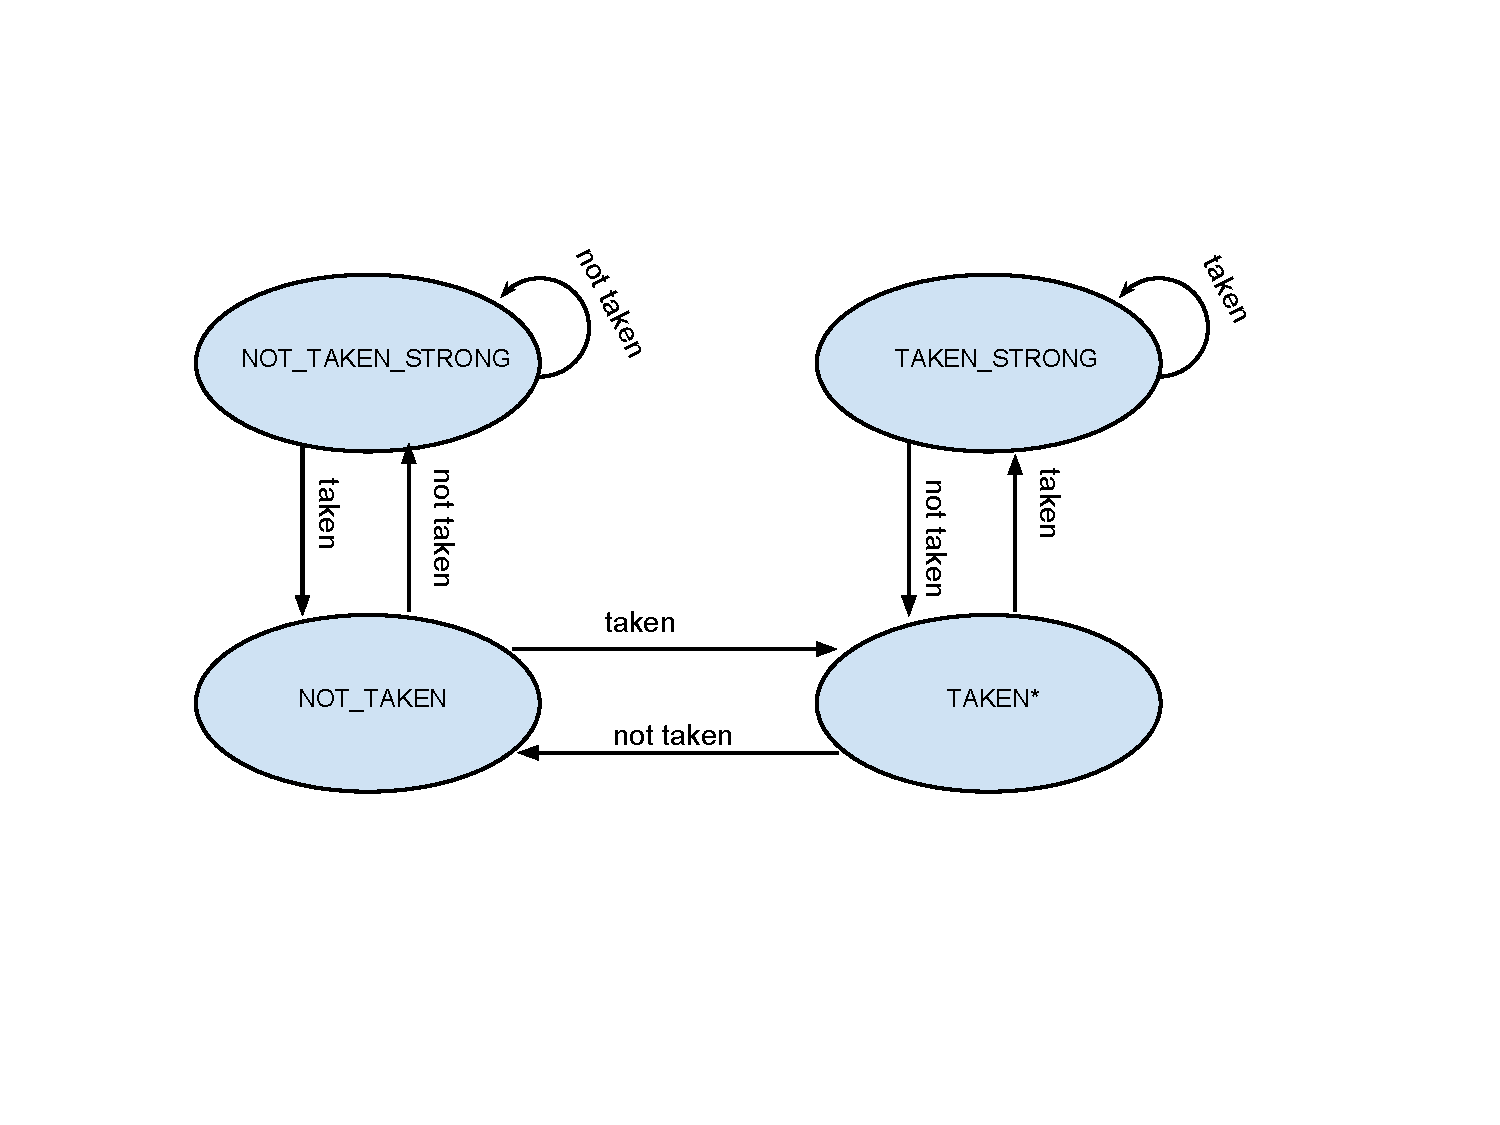
\includegraphics[scale=0.5]{figures/BPU_state_machine}
        \caption{BPU - state machine states and transitions}
        \label{fig:bpu_state_machine}
\end{figure}

As a final note it is worth mentioning that in order to get the BPU states to
synthesize as RAM on the chip the BPU had to be built fully synchronous,
even though the predicted terminals theoretically could have been 
asynchronous. Because of this the BPU gets its two address inputs, predict
and correct, from the stage one step earlier than where they theorically
should have come from. Predict is read from the instruction fetch stage, while correct is read from the instruction decode stage. But
because the BPU is synchronous logically the addresses come from the
ID and EX stages repectivly as the value read from the actual stages are
clocked into the theoretically correct stages as they are clocked into the
BPU.